\documentclass[12pt, a4paper]{article} 
 
\usepackage[utf8]{inputenc}
 

\usepackage[bottom = 8em]{geometry} % to change the page dimensions
\geometry{a4paper} % or letterpaper (US) or a5paper or....
 
\usepackage{graphicx} % support the \includegraphics command and options
\usepackage{grffile}
 
\usepackage{booktabs} % for much better looking tables
\usepackage{array} % for better arrays (eg matrices) in maths
\usepackage{float}
\usepackage{paralist} % very flexible & customisable lists (eg. enumerate/itemize, etc.)
\usepackage{verbatim} % adds environment for commenting out blocks of text & for better verbatim
\usepackage{subfig} % make it possible to include more than one captioned figure/table in a single float
% These packages are all incorporated in the memoir class to one degree or another...
 
 
 
\usepackage{amsmath, amssymb}% for mathematical symbols
\usepackage[colorlinks=true,linkcolor=black]{hyperref} % for hyperreferences with black color
%\usepackage[T1]{fontenc} % Uncomment for norwegian document
%\usepackage[norsk]{babel} %
 
%%% HEADERS & FOOTERS
\usepackage{fancyhdr} % This should be set AFTER setting up the page geometry
\pagestyle{fancy} % options: empty , plain , fancy
\renewcommand{\headrulewidth}{0pt} % customise the layout...
\lhead{}\chead{}\rhead{}
\lfoot{}\cfoot{\thepage}\rfoot{}

 
%%% SECTION TITLE APPEARANCE
\usepackage{sectsty}
\allsectionsfont{\sffamily\mdseries\upshape} % (See the fntguide.pdf for font help)
% (This matches ConTeXt defaults)
 
%%% ToC (table of contents) APPEARANCE
\usepackage[nottoc,notlof,notlot]{tocbibind} % Put the bibliography in the ToC
\usepackage[titles,subfigure]{tocloft} % Alter the style of the Table of Contents
\renewcommand{\cftsecfont}{\rmfamily\mdseries\upshape}
\renewcommand{\cftsecpagefont}{\rmfamily\mdseries\upshape} % No bold!
 
 
%%% END Article customizations
 
%%% The "real" document content comes below...
 
\title{Subsymbolic AI assignment 4}
\author{Eivind Hærum \& \ Hong-Dang Lam}
\date{\today} % Activate to display a given date or no date (if empty),
         % otherwise the current date is printed 
 
\begin{document}
\pagenumbering{gobble}
\maketitle
%\begin{abstract}
% 
%Abstract
% 
%\end{abstract}
\newpage

\tableofcontents
\pagenumbering{roman}
\newpage

\section{Overview of system}
\pagenumbering{arabic}
The genoType is represented as an array of integers, where there is allotted space for all the weights between the nodes, and then 3x the number of nonInput nodes, for bias, gain and timestep. The ranges of these integers are [-5000, 5000] for the weights, [-10000, 0] for the bias, [1000, 5000] for gain and [1000, 2000] for timestep. What PhenoType then does is divide each value in the genotype by 1000.0 netting a array of doubles with real numbers that can be floating point numbers, i.e. possible to use as weights. To make sure that the values does not get mixed up in crossover or mutation, the code  specifically checks which position of the genotype array we are trying to change and make seperate possible outcomes based upon what is supposed to be at a particullar spot, i.e. the ranges for the specific weight type. 


The Beer Agent is an agent with 5 sensors which is able to detect a falling block if and only if part of the block is above one of its 5 sensors. Whenever the sensors detects a block the agent will be lighting up that particular sensor (turning it blue).
The scenarios are made by randomly spawning a block of width [1, 6] at some random position along the x-axis. The blocks fall with a vertical speed of 1, and a horizontal speed of either -1, 0 or 1. Meaning they can fall straight or sideways.

The CTRNN is made up by 5 inputs, which corresponds to the agent's sensors which will give a 1 or 0 depending on if the sensors can sense a block or not. There's currently no layers of hidden nodes, as we cannot get the agent to act in any intelligent manner when these are enabled, thus we have direct mapping, but with the use of bias, gain and timestep for the output nodes (in essence for all nodes that are not input nodes, so with a hidden layer each node has its own values). The values emitted all beyond the input nodes are denoted $ O_i $. The values $ O_i $ are stored for the next round, which is used as input to the other nodes in the same layer (including itself).
The output from the left motor and right motor is something between 0 and 1. The agent gets the output from these motors and compares them, if they are similar, the agent will stay put. If left is larger than the right output, it will move left with $ 5*leftMotorOutput() $, this gives us a move from 0 to 4 positions. That means that even if the left motor output is larger than the right one, it can still stand still if the values is small enough. The same applies if the right output is larger than the left one.

\section{verifying catching}

The agent is able to connect with all the falling blocks even when we don't use any hidden layers. The agent will always move in one direction until it finds a block, it will then try to align itself with that block to catch it. Sometimes it finds out that the best thing to do is to align the block to the side of itself - this happens mostly when the blocks are of a bigger size. The agent believes that the block it's currently sensing is a small one because only 3 of its sensors are detecting the block, but the the truth is that the rest of the block is outside of its range. This behaviour doesn't affect smaller blocks (3 or less in size) that much, because the block is still inside the agent when it reached the bottom.

\begin{figure}[H]
	\begin{center}
		\begin{tabular}{l | c | c |c |c |c |c |c |c|c|c}
		 Contacted& 40&39&39&40&40&40&37&38&33&40\\ \hline
		 Captured & 40&38&36&36&33&40&35&38&33&38\\
		 \\
		 Contacted &36&40&40&40&37&40&40&37&40&39\\ \hline
		 Captured &33&36&35&35&36&37&34&34&39&38\\

		\end{tabular}
	\end{center}
\end{figure}
The table shows number of blocks that the agent have been in contact with and how many it have captured (the whole block is being on top of the agent). The maximum number of blocks spawned is 40.

The Fitness function used is: 
\begin{verbatim}
if captures==0:
    return -1
else:
    return
	\end{verbatim}
    $$\frac{captures}{total}-\frac{contacts-captures}{total}$$

The original function intended for both capture and avoidance makes a bigger emphasis on avoiding big blocks and promptly punishes quite hard for those events, but as all we care about here is capturing all the blocks this is sufficient. The idea about this current function is that we reward the agent whenever it properly catches a block, and subtract any instances where the agent is in contact with a block but is unable to catch it. 



\section{catching and avoiding}
The agent's strategy in this case is to stand still until it senses a block falling. If the block is considered a small block, it will try to go after it and catch it. If it's a big block on the other hand, it will avoid it. The agent doesn't search for new blocks though, this is because the agent is staying put whenever there's no sensor values. It seems very much so that the agent is hindered by the lack of a hidden layer which could make sense of the more complex scenarios, too bad the implementation with hidden layers seem to struck out. 

A fitness run of a decent run looks like this:
\begin{figure}
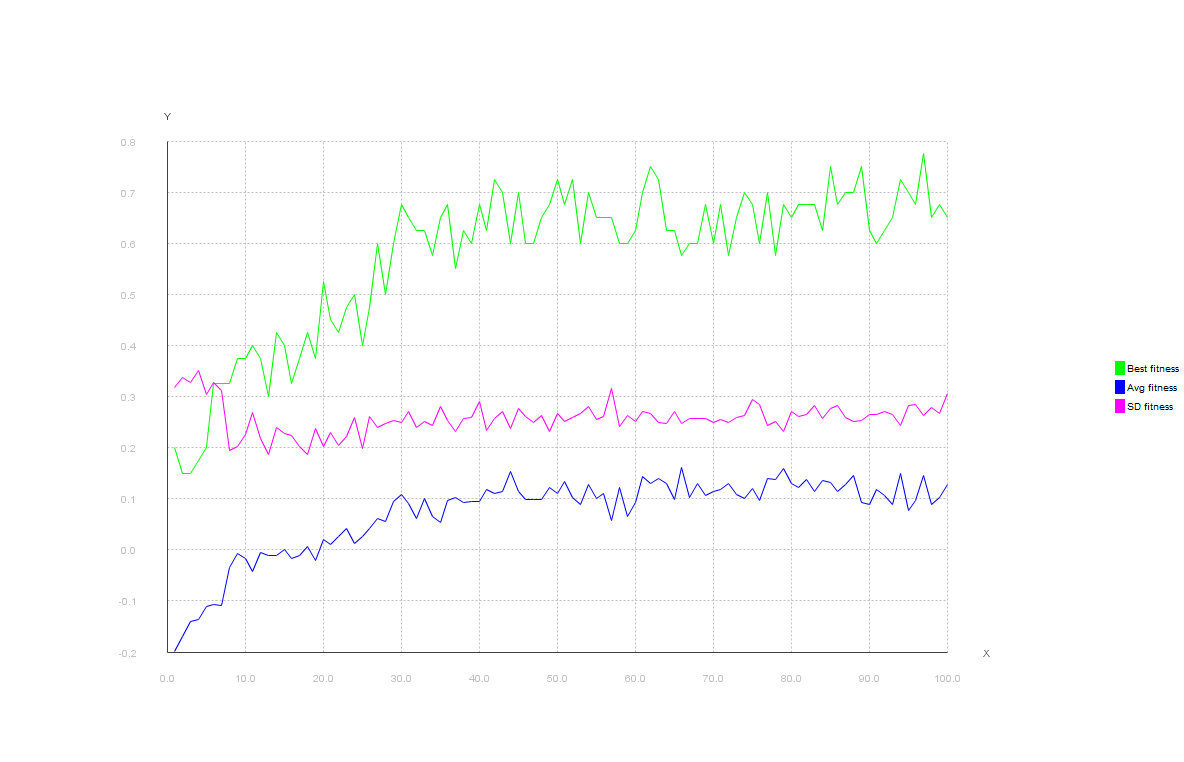
\includegraphics{catch_avoid_dump}
\end{figure}

The results table looks like this:

%%insert shit her:
\begin{figure}[H]
	\begin{center}
		\begin{tabular}{l | c | c |c |c |c }
		 Contacted& 9 & 36 & 27 & 36 & 25\\ \hline
		 Captured & 6 & 21 & 21 & 31 & 23\\
		 
		\end{tabular}
	\end{center}
	\caption{Results of avoid and capture}
\end{figure}




\section{one significant modification of tracker}
We tried to interpret the motor output in a different way, instead of checking the left and the right motor output against each other. Instead of comparing the left and right output, we simply use the formula:\\ $numberOfMoves = \lfloor 4*rightOutput()+1 \rfloor - \lfloor 4*leftOutput()+1 \rfloor$
and then set the position of as: $ poisiton + numberOfMoves $.

\section{one significant modification of ANN topology}
Currently we don't use a hidden layer at all, that's what seems to work the best. If we try to add the hidden layers (1 layer and 2 nodes) then the best overall fitness is around 0.25. The output nodes give very small numbers, so the agent ends up standing still most of the time. The best overall fitness without the hidden layer is 0.975. Thus any changes in regard to the number of hidden nodes, i.e. adding such, do not end up providing better results.

\section{one significant modification of EA variable}
Attempting to change for example the weight range from [-5,5] to [-7,7] seem to have some impact on the avoid \& catch scenario, but this is again without the use of hidden layers. The results for avoid and capture ends up like this:

\begin{figure}[H]
	\begin{center}
		\begin{tabular}{l | c | c |c |c |c }
		 Contacted& 9 & 36 & 27 & 36 & 25\\ \hline
		 Captured & 6 & 21 & 21 & 31 & 23\\
		 
		\end{tabular}
	\end{center}
	\caption{Results of avoid and capture with weight range[-7,7]}
\end{figure}

Here we see that it is still possible to be very unlucky and very lucky as we have as few as 6 blocks captured and as many as 31, the bevhaiour still isnt flawless, it somewhat regurarly still attempts to capture the big blocks. 

\section{detailed analysis}

\end{document}
